% ============================================================
%  CAPITOLO 3 -- PRESA D'ARIA A DOPPIA RAMPA
% ============================================================
\chapter{Presa d'Aria a Doppia Rampa}
\label{cap:doppia_presa}

\section{Descrizione del Caso Studio}
\label{sec:presa_descrizione}

Il secondo caso studio analizzato è una \textbf{presa d'aria supersonica a doppia rampa} (\textit{double-ramp inlet}), tipica dei sistemi propulsivi per velivoli supersonici.

Il principio di funzionamento si basa sul fatto che una rampa inclinata rispetto al flusso
genera un \emph{urto obliquo} attaccato al bordo della rampa stessa. Attraverso l'urto la
corrente viene compressa isentropicamente (in prima approssimazione) e deflessa.
Con \emph{due} rampe di inclinazione crescente si ottengono due urti obliqui successivi:
il primo comprime moderatamente la corrente, il secondo comprime ulteriormente il flusso già
rallentato; il risultato è un processo di compressione più efficiente rispetto a un singolo
urto, con perdite di pressione totale minori.

Le condizioni operative sono:
\begin{itemize}
  \item Numero di Mach di ingresso: $M_{\rm in} = 3$ (regime supersonico)
  \item Angolo di attacco: $\alpha = 0°$ (flusso parallelo all'asse $x$)
  \item Il flusso in uscita è supersonico, pertanto la condizione di pressione statica
    all'outlet non è applicata (la corrente non ha caratteristiche entranti dal bordo destro).
\end{itemize}

\begin{figure}[H]
  \centering
  \begin{tikzpicture}[scale=4.2, >=Stealth]
    % --- Dominio (riempimento) ---
    \fill[blue!5] (-0.5,0) -- (-0.5,0.8) -- (0.832,0.8) -- (0.832,0.426)
      -- (0.617,0.280) -- (0.797,0.310) -- (1,0.310) -- (1,0.204)
      -- (0.720,0.207) -- (0.353,0.0623) -- (0,0) -- (-0.45,0) -- (-0.5,0) -- cycle;
    % --- Pareti solide (Wall): rampe, fondo canale e labbro ---
    \draw[very thick, gray!75] (-0.5,0) -- (0,0);
    \draw[very thick, gray!75] (0,0) -- (0.353,0.0623);          % 1a rampa
    \draw[very thick, gray!75] (0.353,0.0623) -- (0.720,0.207);  % 2a rampa
    \draw[very thick, gray!75] (0.720,0.207) -- (1,0.204);       % fondo canale
    \draw[very thick, gray!75] (0.832,0.8) -- (0.832,0.426) -- (0.617,0.280); % bordo esterno labbro
    \draw[very thick, gray!75] (0.617,0.280) -- (0.797,0.310) -- (1,0.310);   % labbro interno
    % --- Simmetria / far-field (bordo superiore) ---
    \draw[very thick, blue!45!black, dash dot] (-0.5,0.8) -- (0.832,0.8);
    % --- Inlet (sinistra) ---
    \draw[very thick, green!55!black] (-0.5,0) -- (-0.5,0.8);
    % --- Outlet (destra) ---
    \draw[very thick, red!65!black] (1,0.204) -- (1,0.310);
    % --- Urti obliqui: convergono verso il labbro (spigolo all'imbocco del canale).
    %     L'inclinazione mostrata vale per M=3: a Mach piu' alti gli urti si "sdraiano". ---
    \coordinate (lip) at (0.617,0.280);
    \draw[dashed, orange!85!black, thick] (0,0) -- (lip);          % urto 1 (1a rampa)
    \draw[dashed, red!70!black, thick]    (0.353,0.0623) -- (lip); % urto 2 (piu' inclinato)
    % --- Frecce del flusso a monte ---
    \foreach \y in {0.2, 0.4, 0.6}
      \draw[->, blue!55, thick] (-0.64,\y) -- (-0.5,\y);
    \node[left, blue!55, font=\footnotesize] at (-0.64,0.4) {$M_\infty = 3$};
    % --- Etichette dei contorni (leggibili) ---
    \node[above, green!55!black, font=\footnotesize] at (-0.5,0.8) {Inlet};
    \node[below right, red!65!black, font=\footnotesize] at (1,0.31) {Outlet};
    \node[above, blue!45!black, font=\footnotesize] at (0.16,0.8) {Simmetria / far-field};
    \node[below, gray!45!black, font=\footnotesize] at (-0.25,0.0) {Wall};
    \node[right, gray!45!black, font=\footnotesize] at (0.84,0.45) {Wall (labbro)};
    % --- Etichette rampe ---
    \node[below, font=\tiny] at (0.18,0.02) {1\textordfeminine{} rampa};
    \node[below, font=\tiny] at (0.55,0.135) {2\textordfeminine{} rampa};
    % --- Etichette urti (allineate alle linee) ---
    \node[orange!85!black, font=\tiny, rotate=25, anchor=south] at (0.18,0.084) {urto 1};
    \node[red!70!black, font=\tiny, rotate=40, anchor=south] at (0.45,0.142) {urto 2};
    \node[font=\tiny, anchor=west] at (0.63,0.265) {labbro};
  \end{tikzpicture}
  \caption{Schema del dominio computazionale per la presa a doppia rampa (non in scala).
           Le linee tratteggiate indicano gli urti obliqui attesi, che si originano dal piede
           della prima rampa e dal ginocchio della seconda e \textbf{convergono verso il labbro}
           all'imbocco del canale di uscita. L'inclinazione mostrata è quella relativa a
           $M_\infty = 3$: poiché l'angolo dell'onda d'urto dipende dal numero di Mach, a Mach
           più elevati gli urti si "sdraiano" (angolo minore) e il punto di intersezione si
           sposta. Sono indicati i bordi di \textbf{Inlet}, \textbf{Outlet}, \textbf{Wall}
           (pareti solide) e \textbf{Simmetria/far-field} (bordo superiore).}
  \label{fig:dominio_presa}
\end{figure}

\section{Condizioni di Inlet e Outlet}

\begin{table}[h!]
\centering
\begin{tabular}{|l|l|l|}
\hline
 & \textbf{Inlet} & \textbf{Outlet} \\ \hline
\textbf{$T^\circ$} & 1 & - \\ \hline
\textbf{$p^\circ$} & 1 & - \\ \hline
\textbf{p} & - & 0.001 \\ \hline
\textbf{M} & 3 & - \\ \hline
\textbf{Alpha} & $0^\circ$ & - \\ \hline
\end{tabular}
\caption{Condizioni di Inlet e Outlet - Presa a Doppia Rampa}
\label{tab:doppia_rampa_conditions}
\end{table}

\section{Geometria -- Versione Reale e Semplificata}
\label{sec:presa_geometrie}
La modellazione della presa a doppia rampa presenta insidie legate alla complessa interazione fluidodinamica degli urti obliqui. Dal punto di vista fisico, il flusso incontra due rampe successive. Ciascuna rampa genera un'onda d'urto obliqua. Poiché la seconda rampa si trova a valle e ha un'inclinazione maggiore, l'urto generato da essa tende ad intersecare il primo urto in una certa regione del dominio. A rigore, si forma anche un terzo urto obliquo in corrispondenza del labbro della presa (il "cuneo" al punto 9), che va a sommarsi a questo complesso sistema di interazioni.

La posizione esatta in cui questi urti si incontrano dipende fortemente dal \textbf{numero di Mach in ingresso}. All'aumentare del Mach, gli urti obliqui si "sdraiano" maggiormente (l'angolo dell'onda diminuisce), spostando il punto di intersezione più a valle verso l'uscita del dominio.

\paragraph{Il problema del regime subsonico.} 
Poiché la posizione di questa intersezione non è nota a priori senza aver prima risolto il campo, modellare l'intero dominio originale espone a un rischio numerico severo: a valle dell'intersezione degli urti obliqui, o a causa di un urto normale riflesso, potrebbe generarsi una \textbf{tasca di flusso subsonico}.
Questo cambia radicalmente la natura matematica del problema. Le equazioni di Eulero stazionarie, infatti, sono:
\begin{itemize}
    \item \textbf{Iperboliche} in regime supersonico (le perturbazioni viaggiano in un "cono di Mach" orientato a valle);
    \item \textbf{Ellittiche} in regime subsonico (le perturbazioni si propagano in tutte le direzioni).
\end{itemize}
Di conseguenza, nella regione subsonica le condizioni al contorno (soprattutto all'Outlet) andrebbero gestite in modo completamente diverso (imponendo la pressione statica di uscita e permettendo a un'onda caratteristica di rientrare nel dominio). 

\paragraph{La geometria semplificata.}
Per aggirare questo problema, si ricorre alla \texttt{doppia\_presa\_semplificata.geo}. Questa geometria taglia verticalmente il dominio \emph{prima} della zona di complessa interazione degli urti e della sezione interna problematica (chiudendo tra il labbro e il tetto). Ignorando la regione a valle del punto 9, garantiamo che l'intero dominio di calcolo rimanga in regime supersonico, permettendoci di imporre l'estrapolazione di tutte le variabili all'Outlet.

\paragraph{Zone critiche per il raffinamento.}
Alla luce di queste considerazioni, l'infittimento della mesh non deve essere uniforme. Nel campo non strutturato semplificato si è scelto di usare un \emph{Attractor} focalizzato su:
\begin{itemize}
    \item \textbf{Le due rampe (linee 3 e 4)}: ostacoli fisici che innescano variazioni discontinue (forti gradienti);
    \item \textbf{Il labbro e la parte terminale (linee 7 e 8)}: per catturare la formazione del terzo urto e le condizioni di cattura della presa d'aria.
\end{itemize}
Al contrario, regioni come l'angolo superiore sinistro (Inlet-alto, vicino al punto 12) rappresentano il flusso a monte indisturbato e non necessitano di una risoluzione spinta. 
Sono stati prodotti due file \texttt{.geo} distinti:
\begin{itemize}
  \item \texttt{doppia\_presa\_reale.geo}: geometria completa con il condotto di cattura
    e la zona di uscita doppie (include la regione di separazione interna).
  \item \texttt{doppia\_presa\_semplificata.geo}: versione semplificata con chiusura diretta
    del dominio e raffinamento mesh ottimizzato per le simulazioni CFD.
\end{itemize}

\subsection{Geometria Reale}
\label{sec:presa_reale}

Geometria completa, file \texttt{doppia\_presa\_reale.geo}.

\begin{lstlisting}[style=gmsh, caption={File \texttt{doppia\_presa\_reale.geo} -- geometria completa.}, label={lst:presa_reale}]
Mesh.MshFileVersion = 2.2;

// --- Lunghezza caratteristica globale (scalata sull'unita') ---
lc = 1;

// ============================================================
// Definizione dei 12 punti della geometria
// ============================================================
// --- Linea di simmetria/fondo: punti da sinistra verso destra ---
Point(1)  = {-0.500, 0,      0, lc}; // angolo inf. sinistro (Inlet-basso)
Point(2)  = {-0.450, 0,      0, lc}; // bordo anteriore della prima rampa
Point(3)  = {0,      0,      0, lc}; // piede della prima rampa (origine)
Point(4)  = {0.353,  0.0623, 0, lc}; // ginocchio tra prima e seconda rampa
                                      // pendenza 1a rampa: atan(0.0623/0.353)~10deg
Point(5)  = {0.720,  0.207,  0, lc}; // ginocchio tra seconda rampa e fondo canale
                                      // pendenza 2a rampa: atan((0.207-0.0623)/(0.720-0.353))~21.4deg
Point(6)  = {1,      0.204,  0, lc}; // fondo del canale lato uscita (Outlet inf.)
// --- Bordo superiore del canale ---
Point(7)  = {1,      0.310,  0, lc}; // angolo sup. destro (Outlet sup.)
Point(8)  = {0.797,  0.310,  0, lc}; // inizio del labbro superiore interno
Point(9)  = {0.617,  0.280,  0, lc}; // bordo di cattura della presa (labbro)
// --- Bordo superiore esterno ---
Point(10) = {0.832,  0.426,  0, lc}; // angolo del bordo esterno superiore
Point(11) = {0.832,  0.800,  0, lc}; // angolo sup. dell'esterno
Point(12) = {-0.500, 0.800,  0, lc}; // angolo sup. sinistro (Inlet-alto)

// ============================================================
// Definizione delle 12 linee del contorno
// ============================================================
Line(1)  = {1,  2};  // piano d'ingresso inferiore (orizzontale)
Line(2)  = {2,  3};  // zona piatta davanti alla prima rampa
Line(3)  = {3,  4};  // prima rampa (pendenza ~10 deg)
Line(4)  = {4,  5};  // seconda rampa (pendenza ~21 deg)
Line(5)  = {5,  6};  // fondo orizzontale del canale
Line(6)  = {6,  7};  // bordo destro del canale (Outlet)
Line(7)  = {7,  8};  // bordo superiore del canale (uscita)
Line(8)  = {8,  9};  // labbro superiore della presa
Line(9)  = {9,  10}; // bordo esterno del labbro
Line(10) = {10, 11}; // bordo esterno verticale
Line(11) = {11, 12}; // bordo superiore esterno (orizzontale)
Line(12) = {12, 1};  // Inlet (bordo sinistro verticale)

// --- Chiusura del contorno e superficie ---
Line Loop(1) = {1,2,3,4,5,6,7,8,9,10,11,12};
Plane Surface(1) = {1};
\end{lstlisting}

\paragraph{Note sulla geometria reale.}
La geometria include 12 punti e 12 linee che descrivono il profilo esterno della presa, il
canale interno e la zona di uscita. I punti chiave sono:
\begin{itemize}
  \item \textbf{Punti 3--4}: la prima rampa ha pendenza
    $\arctan(0.0623/0.353) \approx 10°$ rispetto all'orizzontale.
  \item \textbf{Punti 4--5}: la seconda rampa ha pendenza
    $\arctan\!\left(\frac{0.207-0.0623}{0.720-0.353}\right) \approx 21.4°$.
  \item \textbf{Punto 9}: il \emph{labbro} della presa, che separa il flusso catturato da
    quello che scorre esternamente.
  \item \textbf{Punti 10--11}: il bordo superiore esterno che delimita la regione esterna
    del dominio computazionale.
\end{itemize}

\subsection{Geometria Semplificata}
\label{sec:presa_semplificata}

La versione semplificata riduce il numero di punti da 12 a 11, eliminando il punto 10
(bordo esterno superiore) e collegando direttamente il labbro della presa al bordo superiore
del dominio. Questa semplificazione riduce la complessità topologica del dominio senza
alterare la fisica nella zona d'interesse (le rampe e il canale di cattura), e
introduce un raffinamento della mesh ottimizzato per le zone di urto:

\begin{lstlisting}[style=gmsh, caption={File \texttt{doppia\_presa\_semplificata.geo} -- geometria semplificata con raffinamento.}, label={lst:presa_sempl}]
Mesh.MshFileVersion = 2.2;

lc = 1; // lunghezza caratteristica di riferimento

// ============================================================
// 11 punti (vs 12 della versione reale)
// ============================================================
Point(1)  = {-0.500, 0,      0, lc};
Point(2)  = {-0.450, 0,      0, lc};
Point(3)  = {0,      0,      0, lc};
Point(4)  = {0.353,  0.0623, 0, lc};
Point(5)  = {0.720,  0.207,  0, lc};
Point(6)  = {1,      0.204,  0, lc};
Point(7)  = {1,      0.310,  0, lc};
Point(8)  = {0.797,  0.310,  0, lc};
Point(9)  = {0.617,  0.280,  0, lc}; // labbro della presa
// DIFFERENZA rispetto alla versione reale:
// Il punto 10 della versione reale (0.832, 0.426) e' eliminato
Point(10) = {0.617,  0.800,  0, lc}; // direttamente sopra al labbro (stessa x di 9)
Point(11) = {-0.500, 0.800,  0, lc}; // angolo sup. sinistro (= punto 12 della versione reale)

// 11 linee
Line(1)  = {1,  2};
Line(2)  = {2,  3};
Line(3)  = {3,  4};  // prima rampa
Line(4)  = {4,  5};  // seconda rampa
Line(5)  = {5,  6};  // fondo canale
Line(6)  = {6,  7};  // Outlet
Line(7)  = {7,  8};
Line(8)  = {8,  9};  // labbro
Line(9)  = {9,  10}; // chiusura verticale sopra il labbro (semplificazione)
Line(10) = {10, 11}; // tetto
Line(11) = {11, 1};  // Inlet

Line Loop(1) = {1,2,3,4,5,6,7,8,9,10,11};
Plane Surface(1) = {1};

// ============================================================
// MESH NON STRUTTURATA con raffinamento sulle zone di urto
// ============================================================

// --- Campo Attractor: infittisce la mesh vicino alle rampe e al canale ---
Field[1] = Attractor;
// Si attrae la mesh verso le linee geometricamente piu' importanti:
// - Linea 3: prima rampa (genera il primo urto obliquo)
// - Linea 4: seconda rampa (genera il secondo urto obliquo)
// - Linea 5: fondo del canale (gradienti di strato limite)
// - Linea 6: Outlet
// - Linea 7: bordo superiore del canale
// - Linea 8: labbro della presa (geometria critica)
Field[1].EdgesList = {3, 4, 5, 6, 7, 8};

// --- Campo Threshold ---
Field[2] = Threshold;
Field[2].IField  = 1;
// lc nella zona vicina alle rampe: 5% della lunghezza di riferimento
// => elementi piccoli per risolvere gli urti e i gradienti di parete
Field[2].LcMin   = lc * 0.05;  // = 0.05
// lc nella zona lontana dalle rampe: 10% della lunghezza di riferimento
Field[2].LcMax   = lc * 0.10;  // = 0.10
// Distanza di transizione:
// - sotto lc/4 = 0.25 si usa LcMin (zona di urto e parete)
// - oltre lc/2 = 0.50 si usa LcMax (zona indisturbata)
Field[2].DistMin = lc / 4;
Field[2].DistMax = lc / 2;

Background Field = 2;

// Conversione in quadrilateri
Recombine Surface{1};
\end{lstlisting}

\paragraph{Motivazione della semplificazione geometrica.}
La versione semplificata collega direttamente il punto 9 (labbro, coordinate $(0.617, 0.280)$)
al punto $(0.617, 0.800)$ che si trova esattamente sopra di esso sulla stessa verticale.
Questo elimina la rientranza angolata presente nella versione reale (punti 9--10--11), che
avrebbe reso più difficile la generazione di una mesh di qualità in quell'angolo. Dal punto di
vista fisico, la zona modificata è lontana dalle rampe di compressione e non influenza
significativamente la fisica del flusso nella presa.

\paragraph{Motivazione del raffinamento sulle linee 3--8.}
Le linee selezionate come attrattori corrispondono alle zone fisicamente più critiche:
\begin{itemize}
  \item \textbf{Linee 3 e 4} (rampe): qui si attaccano gli urti obliqui. Una mesh fine è
    necessaria per risolvere correttamente la discontinuità di pressione e la deflessione del
    flusso.
  \item \textbf{Linea 5} (fondo del canale): la corrente compressa scorre lungo questa superficie,
    dove si sviluppa uno strato limite anche in assenza di viscosità (nel senso che i gradienti
    normali alla parete sono comunque significativi).
  \item \textbf{Linee 7 e 8} (bordo superiore e labbro della presa): in questa zona gli urti
    riflessi e l'interazione con il labbro producono strutture di flusso complesse che richiedono
    alta risoluzione.
\end{itemize}

Il rapporto $\texttt{LcMax}/\texttt{LcMin} = 2$ garantisce una transizione graduale nella
dimensione delle celle, evitando elementi distorti o con rapporti di aspetto elevati.

\paragraph{Effetto della lunghezza caratteristica sui risultati.}
La scelta della lunghezza caratteristica $l_c$ (e quindi di $\texttt{LcMin}$ nelle zone di urto)
ha un effetto preciso e va motivata. La $l_c$ controlla la \textbf{risoluzione delle
discontinuità}: poiché uno schema ai volumi finiti \emph{spalma} l'urto su alcune celle, una
$l_c$ più piccola produce urti più \textbf{netti} (minore \emph{smearing} numerico) e una
migliore cattura dei gradienti, al prezzo di un numero di celle e di un costo computazionale
maggiori. È importante distinguere due aspetti:
\begin{itemize}
  \item la \textbf{posizione} degli urti obliqui è fissata dalla fisica (relazioni
    $\theta$--$\beta$--$M$) ed è quindi \textbf{sostanzialmente indipendente} da $l_c$: griglie
    diverse collocano gli urti quasi nello stesso punto;
  \item lo \textbf{spessore apparente} dell'urto e l'accuratezza delle grandezze di parete
    (pressione, picchi) \textbf{dipendono} invece da $l_c$: una griglia troppo rada arrotonda i
    salti e sottostima i picchi.
\end{itemize}
Adottare una $l_c$ diversa è quindi legittimo purché la griglia sia \textbf{abbastanza fine da
trovarsi nel regime di convergenza}: in tal caso le grandezze integrali e di parete risultano
indipendenti dalla griglia, mentre l'unica differenza visibile tra una $l_c$ e l'altra è la
maggiore o minore nitidezza con cui vengono risolti gli urti.

\section{Mesh per l'Analisi di Convergenza}
\label{sec:presa_mesh_conv}

L'analisi di convergenza richiede tre griglie progressivamente più fitte. A differenza del bump
(mesh strutturata), per la presa a doppia rampa si impiega una \textbf{mesh non strutturata} a
triangoli, con raffinamento controllato da un campo che infittisce in prossimità delle rampe,
della parete inferiore e del labbro --- cioè dove si formano gli urti e i gradienti maggiori. Le
tre griglie si ottengono \textbf{scalando globalmente} la lunghezza caratteristica $l_c$
($l_c = 1,\ 0.5,\ 0.25$), mantenendo identico lo schema di raffinamento: il raffinamento è
quindi \emph{self-simile}, requisito necessario per l'applicabilità di Richardson alle griglie non
strutturate (cfr.\ Sez.~\ref{subsec:richardson_strutt}).

\begin{table}[H]
  \centering
  \caption{Le tre griglie non strutturate per la convergenza della presa a doppia rampa. L'unico
           parametro che cambia è la lunghezza caratteristica globale $l_c$; il rapporto di
           diradamento sui nodi è $r=(N_{\rm fine}/N_{\rm rada})^{1/2}\approx 2$.}
  \label{tab:presa_mesh}
  \renewcommand{\arraystretch}{1.2}
  \begin{tabular}{cccc}
    \toprule
    Griglia & $l_c$ & $N_{\rm nodi}$ & $h_{\rm eff}\approx\sqrt{A/N}$ \\
    \midrule
    M1 (rada)  & $1.00$ & 4\,320  & $\sim 0.0136$ \\
    M2 (media) & $0.50$ & 16\,564 & $\sim 0.0070$ \\
    M3 (fine)  & $0.25$ & 65\,130 & $\sim 0.0035$ \\
    \bottomrule
  \end{tabular}
\end{table}

\begin{figure}[H]
  \centering
  \begin{minipage}{0.9\textwidth}\centering
    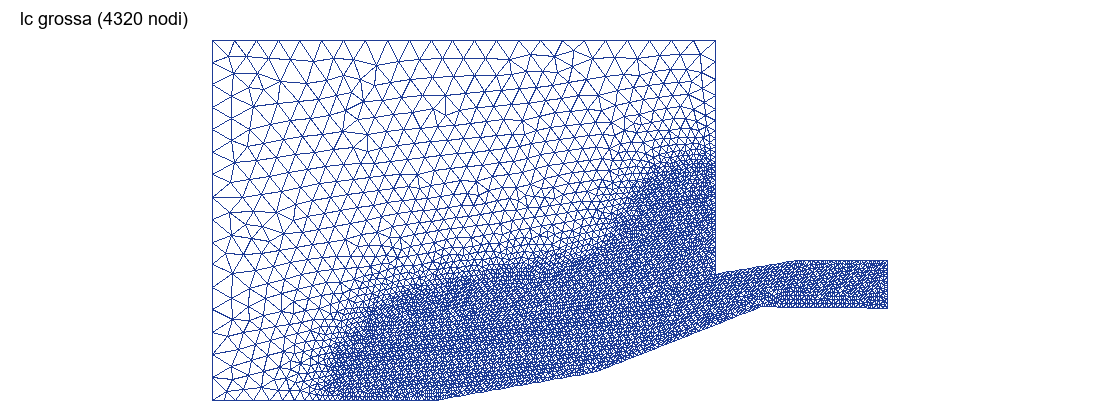
\includegraphics[width=\linewidth]{../Images/mesh_rampa_1.png}\\[-2pt]
    {\footnotesize (a) M1 -- $l_c=1$ -- 4320 nodi}
  \end{minipage}

  \vspace{3pt}
  \begin{minipage}{0.9\textwidth}\centering
    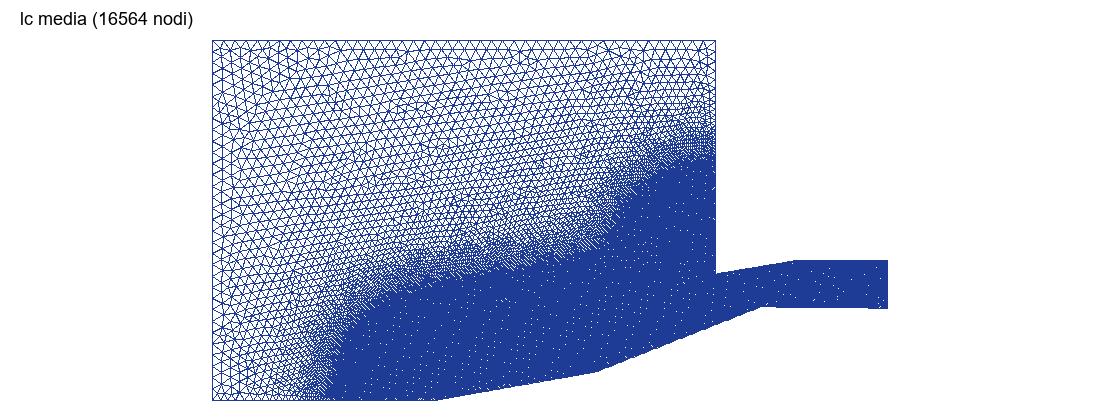
\includegraphics[width=\linewidth]{../Images/mesh_rampa_05.png}\\[-2pt]
    {\footnotesize (b) M2 -- $l_c=0.5$ -- 16564 nodi}
  \end{minipage}

  \vspace{3pt}
  \begin{minipage}{0.9\textwidth}\centering
    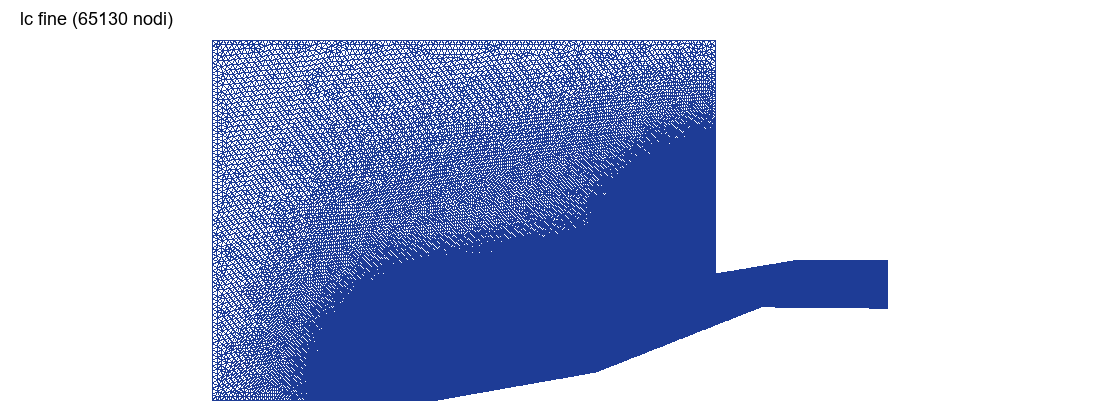
\includegraphics[width=\linewidth]{../Images/mesh_rampa_025.png}\\[-2pt]
    {\footnotesize (c) M3 -- $l_c=0.25$ -- 65130 nodi}
  \end{minipage}
  \caption{Le tre griglie non strutturate a raffinamento crescente per la presa a doppia rampa.
           Si nota l'infittimento concentrato lungo le rampe, la parete inferiore e il labbro,
           dove si sviluppano gli urti obliqui; la zona di monte (flusso indisturbato) resta rada.}
  \label{fig:presa_mesh3}
\end{figure}



\section{Analisi di Convergenza con Estrapolazione di Richardson}
\label{sec:presa_convergenza}

A differenza del bump (subsonico, privo di urti, dove la soluzione esatta è $\bar S=0$), nella
presa a doppia rampa il campo presenta \textbf{urti obliqui fisici}: l'entropia esatta \emph{non}
è nulla (gli urti producono entropia reale) e la stima dell'errore tramite soluzione esatta nota
non è applicabile. Si usa quindi la sola \textbf{estrapolazione di Richardson} (con ordine teorico
ed effettivo), come previsto dalla traccia, impiegando lo schema di \textbf{Roe} sulle tre griglie
non strutturate definite in precedenza.

\paragraph{Scelta della grandezza integrale.}
L'estrapolazione di Richardson richiede una \textbf{singola grandezza scalare} che riassuma l'intero
campo. Si sceglie la \textbf{norma $L_2$ dell'entropia} $\|\bar S\|_2$ (Eq.~\ref{eq:norma_entropia}).
Il suo significato qui è diverso rispetto al bump: non è un errore che tende a zero, ma una grandezza
\emph{integrale} del campo che, al raffinare della griglia, \textbf{converge a un valore non nullo}
--- l'entropia \emph{fisica} prodotta dagli urti --- man mano che si annulla la sola componente
\emph{numerica} (spuria) dovuta alla discretizzazione. Richardson ne stima il valore a griglia
infinita ($u_{\rm esatto}$) e il GCI quantifica quanto la griglia più fine ne sia ancora distante.
È una scelta naturale: l'entropia è massimamente sensibile proprio dove il metodo fatica (gli urti)
ed è già calcolata dal codice come integrale di superficie.

\paragraph{Valori calcolati sulle tre griglie (schema di Roe).}
Eseguendo il codice fino a convergenza dei residui, la norma dell'entropia vale
\begin{equation*}
  u_{h} = 1.443\times10^{-2},\quad
  u_{2h} = 1.651\times10^{-2},\quad
  u_{4h} = 1.973\times10^{-2},
\end{equation*}
dove le tre griglie sono, dalla più fine alla più rada:
$u_{h}\!\to$ M3 ($l_c=0.25$, $65\,130$ nodi), $u_{2h}\!\to$ M2 ($l_c=0.50$, $16\,564$ nodi),
$u_{4h}\!\to$ M1 ($l_c=1.00$, $4\,320$ nodi). Il rapporto di diradamento è $r=2$ (dimezzando $l_c$ il
numero di nodi quadruplica, quindi $r=(N_{\rm fine}/N_{\rm rada})^{1/2}\approx2$).

\begin{table}[H]
  \centering
  \caption{Estrapolazione di Richardson sulla norma $L_2$ dell'entropia -- presa a doppia rampa,
           schema di Roe.}
  \label{tab:presa_convergenza}
  \renewcommand{\arraystretch}{1.3}
  \begin{tabular}{lccccc}
    \toprule
    Metodo & Tipo analisi & $p$ & $u_{\rm esatto}$ & $E$ & GCI \\
    \midrule
    Roe & Ordine teorico   & $1.00$  & $1.236\times10^{-2}$ & $2.08\times10^{-3}$ & $6.23\times10^{-3}$ \\
    Roe & Ordine effettivo & $0.636$ & $1.069\times10^{-2}$ & $3.75\times10^{-3}$ & $1.12\times10^{-2}$ \\
    \bottomrule
  \end{tabular}
\end{table}

\paragraph{Interpretazione.}
\begin{itemize}
  \item La norma dell'entropia \textbf{decresce monotonicamente} al raffinare della griglia
    ($1.97 \to 1.65 \to 1.44 \times 10^{-2}$): la componente numerica si riduce e la grandezza
    converge verso l'entropia fisica degli urti, stimata da Richardson in
    $u_{\rm esatto}\approx1.1$--$1.2\times10^{-2}$.
  \item L'\textbf{ordine effettivo} risulta $p_{\rm eff}\approx0.64$, \emph{inferiore} all'unità:
    è coerente con la presenza di \textbf{urti}, che degradano l'ordine di convergenza degli schemi
    (in corrispondenza di una discontinuità anche uno schema di ordine elevato cade al prim'ordine
    o meno). Le griglie non sono ancora nella regione asintotica piena.
  \item Il \textbf{GCI} sulla griglia più fine è dell'ordine dell'$1\%$ del valore estrapolato:
    indica che la mesh M3 fornisce una soluzione ragionevolmente \emph{grid-independent}, e che già
    la M2 (impiegata per i campi) è prossima alla convergenza --- da cui la scelta di usarla per i
    campi di Mach/pressione/temperatura a costo ridotto.
\end{itemize}

\paragraph{Nota: validità su griglie non strutturate.}
Le tre mesh sono \textbf{non strutturate}, quindi $h$ è una dimensione caratteristica \emph{media} e
il rapporto $r$ è ricavato dal conteggio dei nodi. L'estrapolazione di Richardson resta valida
perché il raffinamento è \textbf{self-simile} --- lo stesso schema di infittimento (medesimi campi
di mesh) applicato globalmente a tutte le griglie, scalando solo $l_c$ --- come discusso nella parte
teorica (Sez.~\ref{subsec:richardson_strutt}).

\section{Condizioni al Contorno e Parametri della Simulazione}
\label{sec:presa_bc}

\begin{table}[H]
  \centering
  \caption{Parametri di simulazione -- presa a doppia rampa.}
  \label{tab:presa_param}
  \begin{tabular}{llll}
    \toprule
    File & Parametro & Valore & Descrizione \\
    \midrule
    \multirow{4}{*}{\texttt{input.txt}}
      & \texttt{KFINAL} & 300\,000 & Iterazioni massime \\
      & \texttt{KINF}   & 100      & Frequenza output a schermo \\
      & \texttt{KOUT}   & 100      & Frequenza salvataggio soluzione \\
      & \texttt{CFL}    & 0.3      & Numero CFL \\
    \midrule
    \multirow{4}{*}{\texttt{inlet.txt}}
      & $T^\circ_{\rm in}$ & 1  & Temperatura totale (adim.) \\
      & $P^\circ_{\rm in}$ & 1  & Pressione totale (adim.) \\
      & $\alpha$           & 0° & Flusso orizzontale \\
      & $M_{\rm in}$       & 3  & Mach supersonico \\
    \midrule
    \texttt{outlet.txt}
      & $P_{\rm exit}$ & 0.001 & Non utilizzato (uscita supersonica) \\
    \bottomrule
  \end{tabular}
\end{table}

\paragraph{Osservazioni sulle condizioni.}
\begin{itemize}
  \item Poiché il flusso è supersonico all'ingresso ($M = 3$), tutte le caratteristiche
    entrano nel dominio da sinistra: si impongono tutte e quattro le variabili conservative.
  \item Con $\text{KINF} = 100$ (anziché 1000 come nel caso bump), la frequenza di output
    è più alta: questo è necessario perché le simulazioni supersoniche convergono molto più
    rapidamente (il dominio è quasi interamente in regime supersonico, e i transitori si
    propagano a velocità elevata attraversando il dominio in poche iterazioni).
  \item Il valore $P_{\rm exit} = 0.001$ è puramente indicativo: in uscita supersonica
    il codice ignora questa condizione e estraprola tutte le variabili dall'interno.
\end{itemize}

\section{Confronto con Dati Sperimentali}
\label{sec:presa_exp}

\begin{figure}[H]
  \centering
  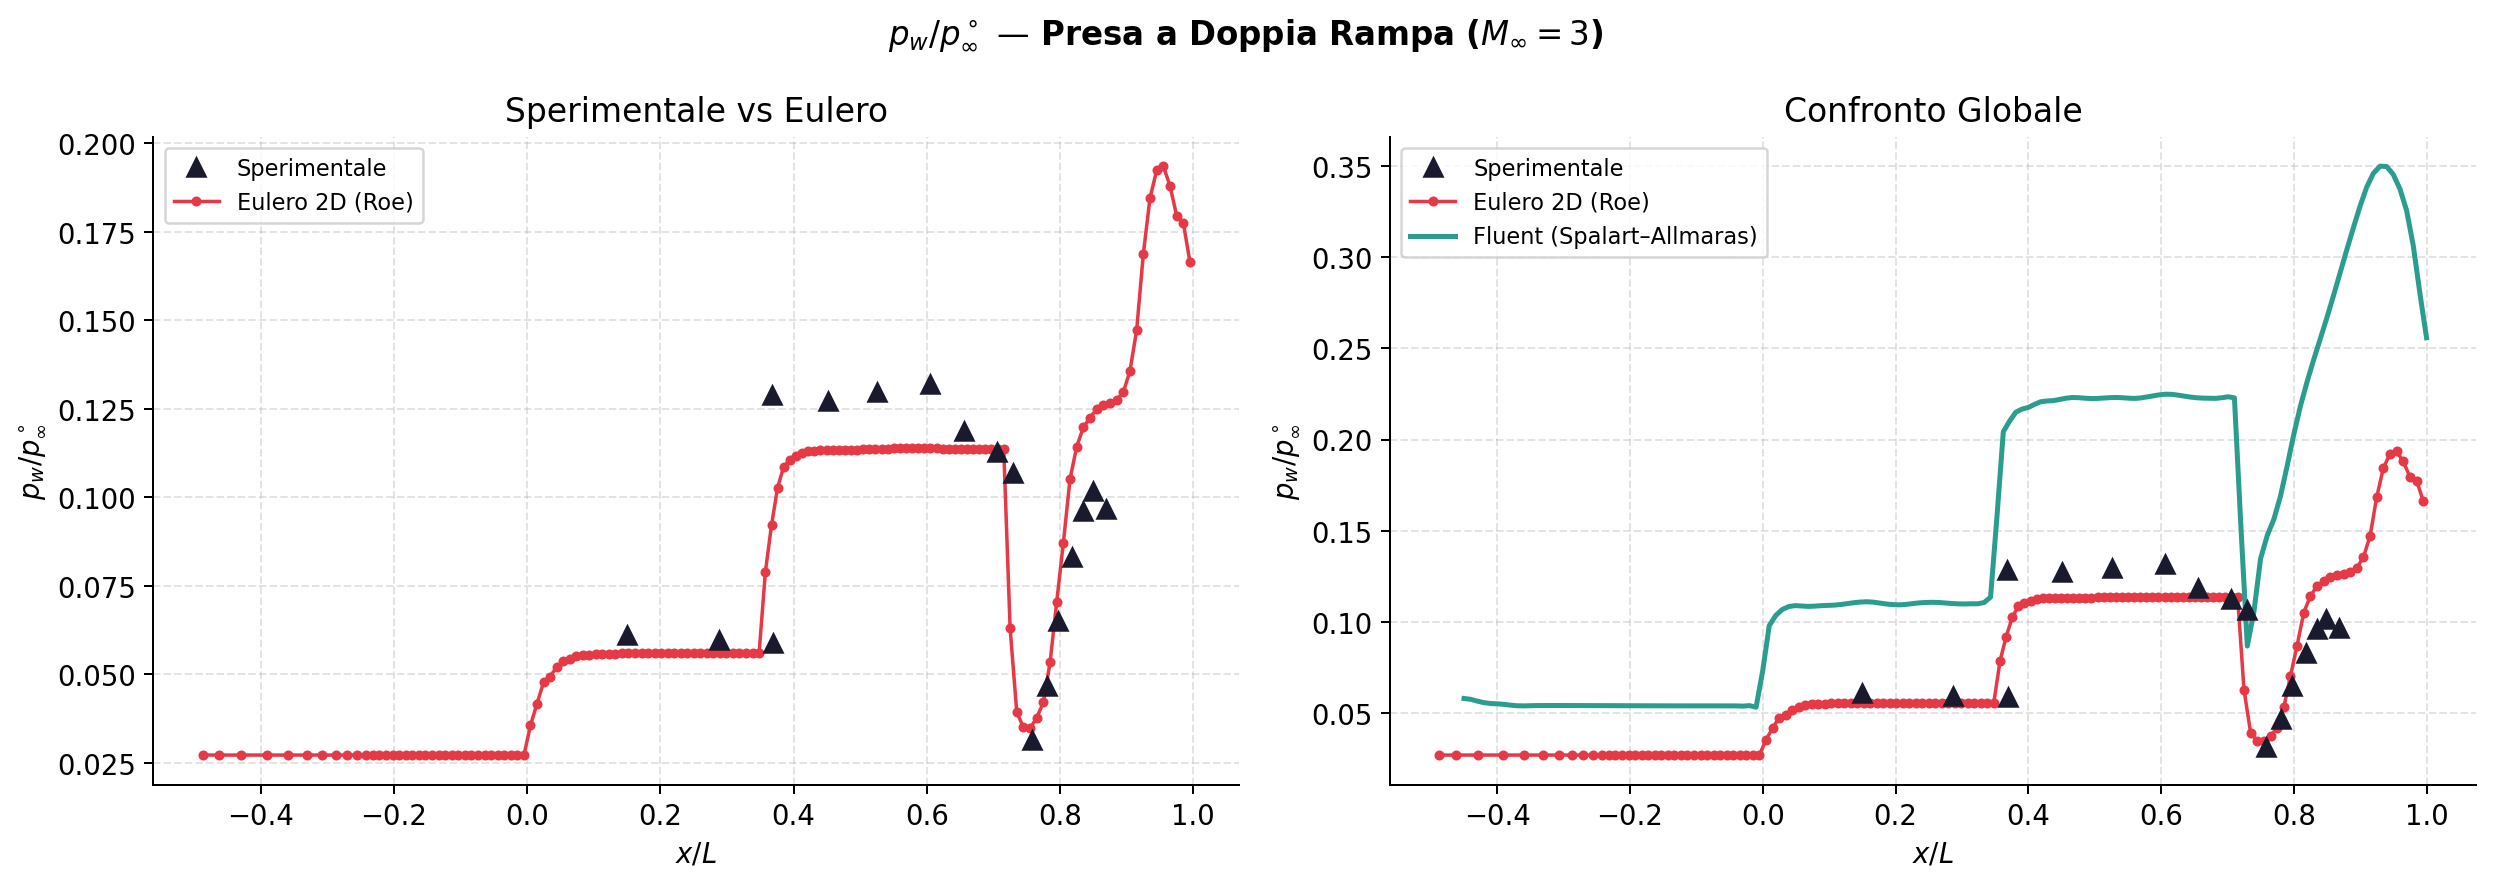
\includegraphics[width=0.85\textwidth]{../Images/confronto_pressione_doppia_rampa}
  \caption{Distribuzione di pressione adimensionale $P_w/P^\circ$ sulla parete inferiore
           della presa a doppia rampa: confronto tra i dati sperimentali, la soluzione Euler
           con schema di Roe (codice sviluppato), la soluzione Euler--CFD (ANSYS Fluent
           inviscido) e il modello RANS Spalart--Allmaras (ANSYS Fluent viscoso).
           I modelli inviscidi sottostimano la distribuzione di pressione a valle degli urti
           per la mancata modellazione dell'interazione urto--strato limite (SBLI), mentre
           il modello RANS con Spalart--Allmaras cattura parzialmente la separazione
           indotta dagli urti, avvicinandosi ai dati sperimentali nella regione downstream.}
  \label{fig:confronto_pressione_doppia_rampa}
\end{figure}

I dati sperimentali disponibili forniscono la distribuzione di pressione sulla parete
inferiore del condotto in funzione della coordinata assiale $x$. Per il confronto si estrae
numericamente la pressione nelle celle di bordo con tag 99 (parete solida), si filtra
per la parete inferiore imponendo una soglia sulla coordinata $y$, e si confronta
$P_w/P^\circ$ con i dati sperimentali.

I risultati mostrano che:
\begin{itemize}
  \item I casi inviscidi (sia il codice sviluppato con schema di Roe sia Fluent inviscido)
    concordano bene tra loro nella distribuzione di pressione;
  \item Le discrepanze maggiori con i dati sperimentali si trovano nella zona a valle degli
    urti ($x > 0.5$), dove il campo è influenzato da interazioni onde d'urto--strato limite
    (SBLI) non catturabili con un modello di Eulero;
  \item Il modello RANS (Fluent viscoso con Spalart--Allmaras) è in grado di cogliere
    parzialmente la separazione indotta dagli urti sulla parete, avvicinandosi maggiormente
    ai dati sperimentali nella regione downstream.
\end{itemize}

% Figura di confronto rimossa perche' duplicata (errore noto #6): la stessa
% immagine confronto_pressione_doppia_rampa con identico \label era inserita due
% volte nella stessa sezione, generando un warning di label multipla. Resta la
% prima occorrenza all'inizio della sezione.

% L'analisi ANSYS Fluent completa (mesh, y+, campi Mach/pressione, strato limite,
% bolla di ricircolo e confronto con dati sperimentali) è trattata nel
% Capitolo~\ref{cap:fluent} dedicato, al fine di evitare duplicazione.

\section{Campi di Mach, Pressione e Temperatura (Solutore Euler)}
\label{sec:presa_campi}

Si presentano infine i campi ottenuti con il \textbf{codice di Eulero sviluppato}, utilizzando lo
\textbf{schema di Roe} come richiesto dalla traccia. La scelta della griglia è guidata
dall'analisi di convergenza: poiché la norma dell'entropia varia poco passando dalla griglia
media (M2) a quella fine (M3), la \textbf{mesh intermedia M2} ($16\,564$ nodi) è già
sufficientemente fitta per fornire risultati attendibili, a un costo computazionale molto
inferiore rispetto alla griglia più fine. I campi sono mostrati a convergenza dei residui.

\paragraph{Verifica delle condizioni di ingresso.}
Prima di interpretare i campi si controlla la consistenza del flusso indisturbato di monte con le
relazioni isentropiche per $M_\infty = 3$:
\begin{equation}
  \frac{T_\infty}{T^\circ} = \left(1+\tfrac{\gamma-1}{2}M_\infty^2\right)^{-1} = \frac{1}{2.8} = 0.357,
  \qquad
  \frac{P_\infty}{P^\circ} = \left(1+\tfrac{\gamma-1}{2}M_\infty^2\right)^{-\frac{\gamma}{\gamma-1}} = 0.0272.
\end{equation}
I valori letti nei campi a monte ($T/T^\circ = 0.357$ e $P/P^\circ = 0.0272$) coincidono
\textbf{esattamente} con questi: le condizioni al contorno sono imposte correttamente e il codice
è consistente.

\begin{figure}[H]
  \centering
  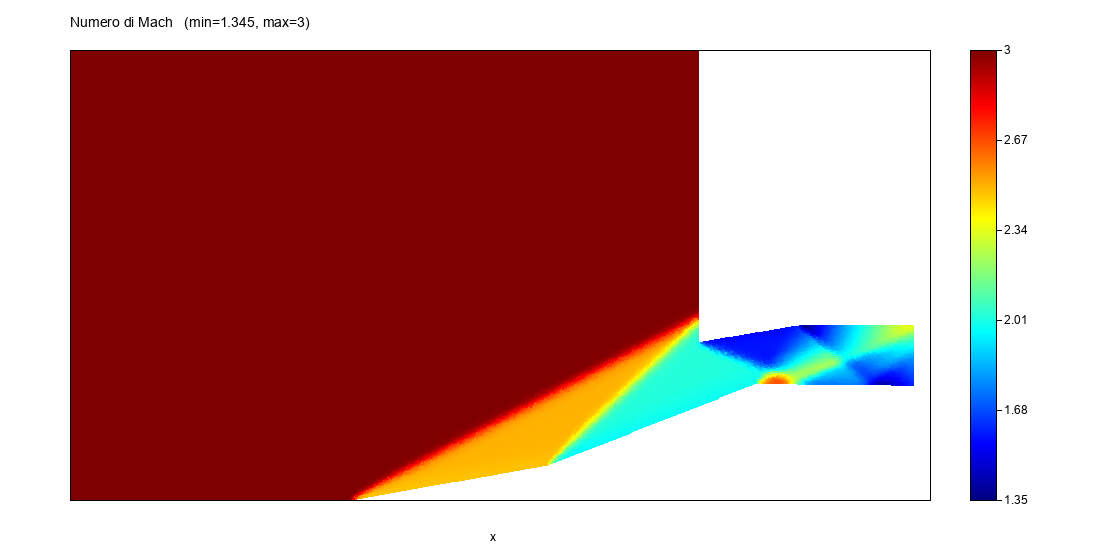
\includegraphics[width=0.92\textwidth]{../Images/Eulero_rampa05_mach.png}
  \caption{Campo del numero di Mach nella presa a doppia rampa (codice Euler, schema di Roe,
           griglia M2). A monte $M=3$ uniforme; i due urti obliqui staccati dalle rampe decelerano
           progressivamente la corrente fino a $M\approx1.35$, mantenendola ovunque
           \textbf{supersonica}. Nel canale si osservano le riflessioni d'onda sulle pareti.}
  \label{fig:eulero_rampa_mach}
\end{figure}

\paragraph{Campo di Mach.}
Il campo riproduce la fisica attesa della presa a compressione esterna:
\begin{itemize}
  \item a monte la corrente è \textbf{uniforme a $M=3$} (regione rossa);
  \item dal piede della prima rampa parte il \textbf{primo urto obliquo}, che deflette e comprime
    il flusso riducendo il Mach; dal ginocchio della seconda rampa parte il \textbf{secondo urto
    obliquo}, più inclinato, che lo riduce ulteriormente;
  \item attraverso la doppia compressione il numero di Mach scende da $3$ a circa $1.35$,
    \textbf{restando supersonico} su tutto il dominio: è esattamente la condizione che la geometria
    semplificata vuole garantire (natura iperbolica delle equazioni, nessuna caratteristica
    entrante dall'outlet);
  \item la \textbf{compressione a due urti deboli} è più efficiente di un singolo urto forte,
    perché la perdita di pressione totale attraverso un urto cresce rapidamente con l'intensità
    ($\Delta P^\circ \propto (M_n^2-1)^3$): due urti deboli dissipano meno di un urto normale unico.
\end{itemize}

\begin{figure}[H]
  \centering
  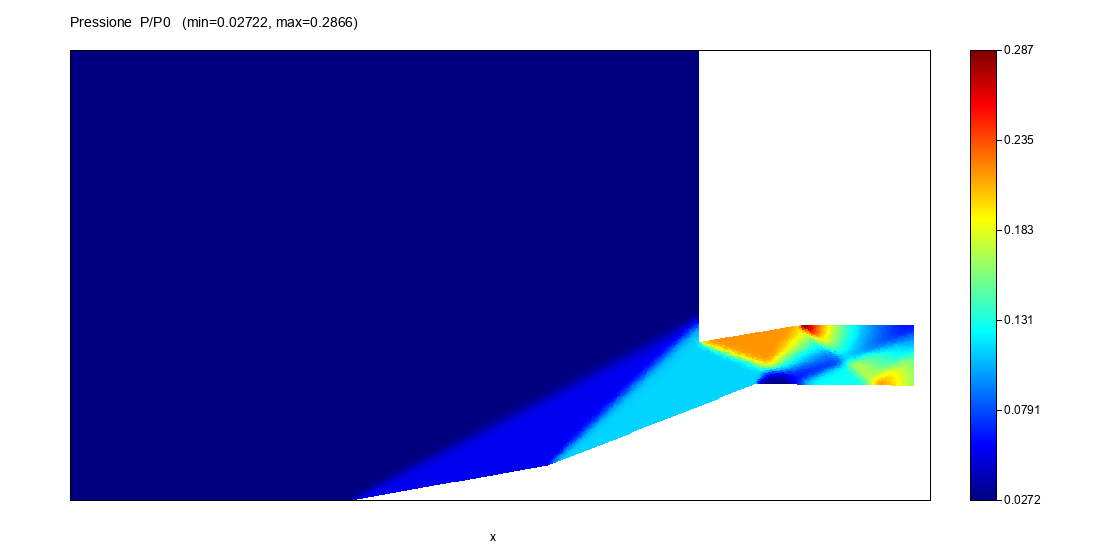
\includegraphics[width=0.92\textwidth]{../Images/Eulero_rampa05_pressione.png}
  \caption{Campo di pressione adimensionale $P/P^\circ$ (codice Euler, schema di Roe, griglia M2).
           Pressione bassa e uniforme a monte ($0.0272$), che cresce a gradini attraverso i due
           urti obliqui fino al picco ($\approx0.29$) nella zona di focalizzazione degli urti
           in prossimità del labbro/imbocco del canale.}
  \label{fig:eulero_rampa_pressione}
\end{figure}

\paragraph{Campo di pressione.}
La pressione statica parte dal valore di monte $0.0272$ e \textbf{cresce a gradini} attraverso i
due urti (ogni urto è una compressione), raggiungendo il \textbf{massimo} ($\approx0.29$, oltre
dieci volte la pressione di monte) nella regione dove i due urti obliqui \textbf{convergono e si
focalizzano} in prossimità del labbro, all'imbocco del canale di cattura. È qui che la presa
realizza il suo scopo: \emph{recuperare pressione} comprimendo la corrente supersonica. A valle,
nel canale, la pressione si ridistribuisce per effetto delle riflessioni d'onda sulle pareti.

\begin{figure}[H]
  \centering
  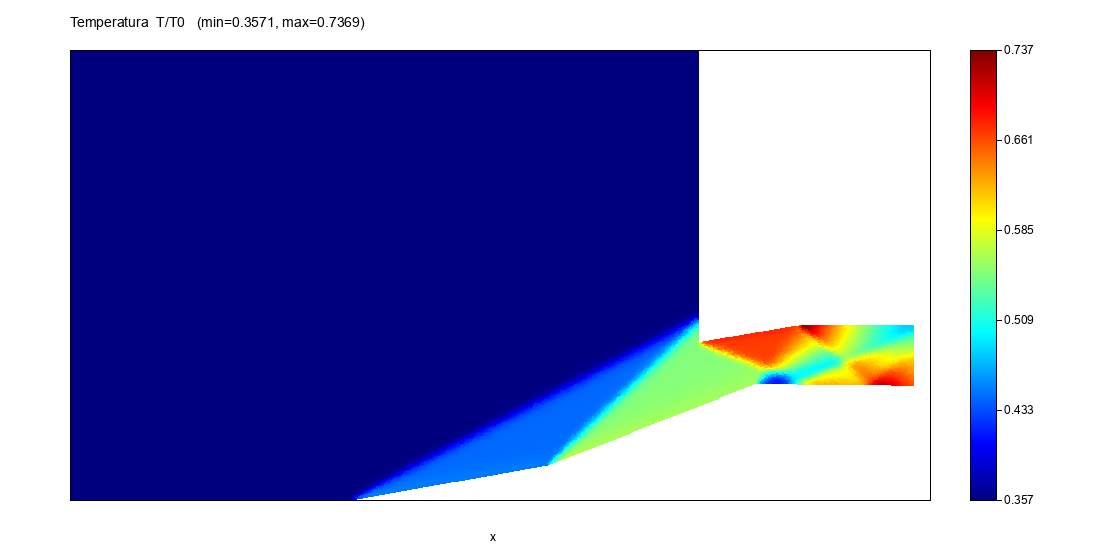
\includegraphics[width=0.92\textwidth]{../Images/Eulero_rampa05_temperatura.png}
  \caption{Campo di temperatura adimensionale $T/T^\circ$ (codice Euler, schema di Roe, griglia M2).
           È l'immagine "speculare" del Mach: minima a monte ($0.357$, flusso veloce) e crescente
           attraverso la compressione fino a $\approx0.74$ nel canale.}
  \label{fig:eulero_rampa_temperatura}
\end{figure}

\paragraph{Campo di temperatura.}
Coerentemente con la relazione isentropica $T/T^\circ=(1+\tfrac{\gamma-1}{2}M^2)^{-1}$, la
temperatura è il \textbf{negativo} del campo di Mach: minima dove il flusso è più veloce (a monte,
$T/T^\circ=0.357$) e crescente attraverso gli urti man mano che la corrente rallenta e si comprime,
fino a $T/T^\circ\approx0.74$ nel canale. La coerenza incrociata fra i tre campi ($M$, $P$, $T$
legati dalle relazioni isentropiche fuori dagli urti) costituisce un'ulteriore validazione del
solutore.

\paragraph{Note sulla risoluzione e sullo schema.}
Rispetto alla griglia più rada, la mesh M2 ($16\,564$ nodi) risolve gli urti in modo
\textbf{nettamente più nitido}, con minore \emph{smearing} numerico. Lo schema di \textbf{Roe},
meno dissipativo, contribuisce alla nitidezza delle discontinuità. Trattandosi di un modello
\textbf{inviscido}, non sono presenti strato limite né separazioni: la bolla di ricircolo e
l'interazione urto--strato limite osservabili nel caso viscoso (Cap.~\ref{cap:fluent}) non
compaiono qui.
